\documentclass[a4paper, 12pt, oneside, openany]{scrbook}

\usepackage[backend=biber,style=alphabetic,citestyle=authoryear ]{biblatex}
\usepackage[ngerman]{babel}
\usepackage[T1]{fontenc}
\usepackage[utf8]{inputenc}
\usepackage[]{hyperref}
\usepackage{graphicx}
\usepackage{epstopdf}
\usepackage{float}
\usepackage{acronym}
\usepackage{booktabs}
\usepackage{caption}
\usepackage{csquotes}
\usepackage{fancyhdr}
\usepackage{url}
\usepackage{listings}
\usepackage{blindtext}
\usepackage{courier}
\usepackage{comment}
\usepackage{pdfpages}
\usepackage{subcaption} 

\newcommand*{\todo}[1]{\colorbox{yellow}{\parbox{1\linewidth} {TODO: #1}}} % Yellow TODO box u.A. https://tex.stackexchange.com/a/319000/129441

\renewcommand*{\headfont}{\normalfont}
%\renewcommand*{\multicitedelim}{\addsemicolon\space}
\renewcommand*{\headrulewidth}{0pt}
\renewcommand*{\arraystretch}{1.5}
\newcommand{\code}{\texttt} % code in monospace font, wont hyphenate https://tex.stackexchange.com/a/36031/129441

\newcommand{\compcite}{\parencite[vgl.][]}

\setlength{\parskip}{1.5ex}

\MakeOuterQuote{"}

\hypersetup{
  colorlinks=true,
  linkcolor=black,
  citecolor=blue,
  urlcolor=cyan
}

% Damit refs automatisch verlinkt werden und "Abb. 1" generiert wird
\usepackage[ngerman]{cleveref}

% "Tabelle 1" wird z.B. zu "Tab. 1" ge�ndert
\addto\captionsngerman{
    \crefname{chapter}{kap.}{kap.}
    \Crefname{chapter}{Kap.}{Kap.}
    \crefname{subsubsection}{abs.}{abs.}
    \Crefname{subsubsection}{Abs.}{Abs.}
    \crefname{subsection}{abs.}{abs.}
    \Crefname{subsection}{Abs.}{Abs.}
    \crefname{section}{abs.}{abs.}
    \Crefname{section}{Abs.}{Abs.}
    \crefname{figure}{abb.}{abb.}
    \Crefname{figure}{Abb.}{Abb.}
    \crefname{table}{tab.}{tab.}
    \Crefname{table}{Tab.}{Tab.}
    \renewcommand{\figurename}{Abb.}
  	\renewcommand{\tablename}{Tab.}
}
% Bibliotheksdatei
\addbibresource{bibliography.bib}

\begin{document}

\frontmatter

\def\title{Entwicklung einer Ernährungsberater-App im Umfeld der Firma Kaufland Informationssysteme GmbH \& Co. KG}
\def\author{Carsten Hagemann}

\begin{titlepage}

\vspace{10mm}

\begin{center}
	\vspace{5mm}
	
	\huge \title{}
	
	\vspace{14.2pt}
	
	\large 1. Praxisarbeit
	
	
	\vspace{42.6pt}
	
	%\small für die Prüfung zum \\
	%\large Bachelor of Science
	
	\vspace{42.6pt}
	
	\small des Studienganges Angewandte Informatik an der \\
	\large Dualen Hochschule Baden-Württemberg Mosbach
    
    \vspace{10.2pt}
    
    
\includegraphics[height=1.5cm]{include/images/logo-dhbw.eps}
    \hspace{35pt}
	
\includegraphics[height=1.5cm]{include/images/kauflandlogo.png}
	
	\vspace{84.6pt}
	
	\small von \\
	\large \author{}
\end{center}

\vspace{68.6pt}

\begin{table}[h]
    \centering
    \begin{tabular}{ll}
        \small Bearbeitungszeitraum                 & 12 Wochen                     \\
        \small Matrikelnummer, Kurs                 & 7694128, INF16B    \\
        \small Ausbildungsfirma                     & Kaufland Informationssysteme GmbH \& Co. KG \\
        \small Betreuer der Ausbildungsfirma        & Maria Lindow        \\
    \end{tabular}
\end{table}

\vspace{49.7pt}

\fancypagestyle{empty}{
  \fancyhf{}
  \fancyfoot[C]{11. September 2017}
}

\end{titlepage}
\chapter*{Sperrvermerk}
Die vorliegende Arbeit beinhaltet interne vertrauliche Informationen der Schwarz-Gruppe. Sie ist nur für die Beteiligten am Begutachtungs- und Evaluationsprozess bestimmt.

Die Weitergabe des Inhalts der Arbeit im Ganzen oder in Teilen daraus an externe Dritte sowie das Anfertigen von Abschriften oder Kopien zu welchem Zweck, in welcher Form und zu welchem Zeitpunkt auch immer ist grundsätzlich untersagt.

Ausnahmen bedürfen der schriftlichen Genehmigung der Firma Kaufland Informationssysteme GmbH \& Co. KG und der Schwarz IT Infrastructure \& Operations Services GmbH \& Co. KG.

Eine Weitergabe an Mitarbeiter der Hochschule aufgrund fachlicher Belange oder für administrative Zwecke ist von dieser Regelung explizit ausgenommen.
\chapter*{Eigenleistung}
Ich versichere hiermit, dass ich meine Praxisarbeit mit dem Thema "\title{}" selbstständig verfasst und keine anderen als die angegebenen Quellen und Hilfsmittel benutzt habe.

\noindent Ich versichere zudem, dass die eingereichte elektronische Fassung mit der gedruckten Fassung übereinstimmt.$^*$

\noindent \small $^*$falls beide Fassungen gefordert sind 

\vspace{30pt}

\line(1, 0){120}  \hspace{60pt}  \line(1, 0){150}

Ort, Datum \hspace{120pt} Unterschrift

% Einzelne PDF-Seite hinzufügen im Dokument.
% Erforderlich für den Ablauf der Praxisphase.
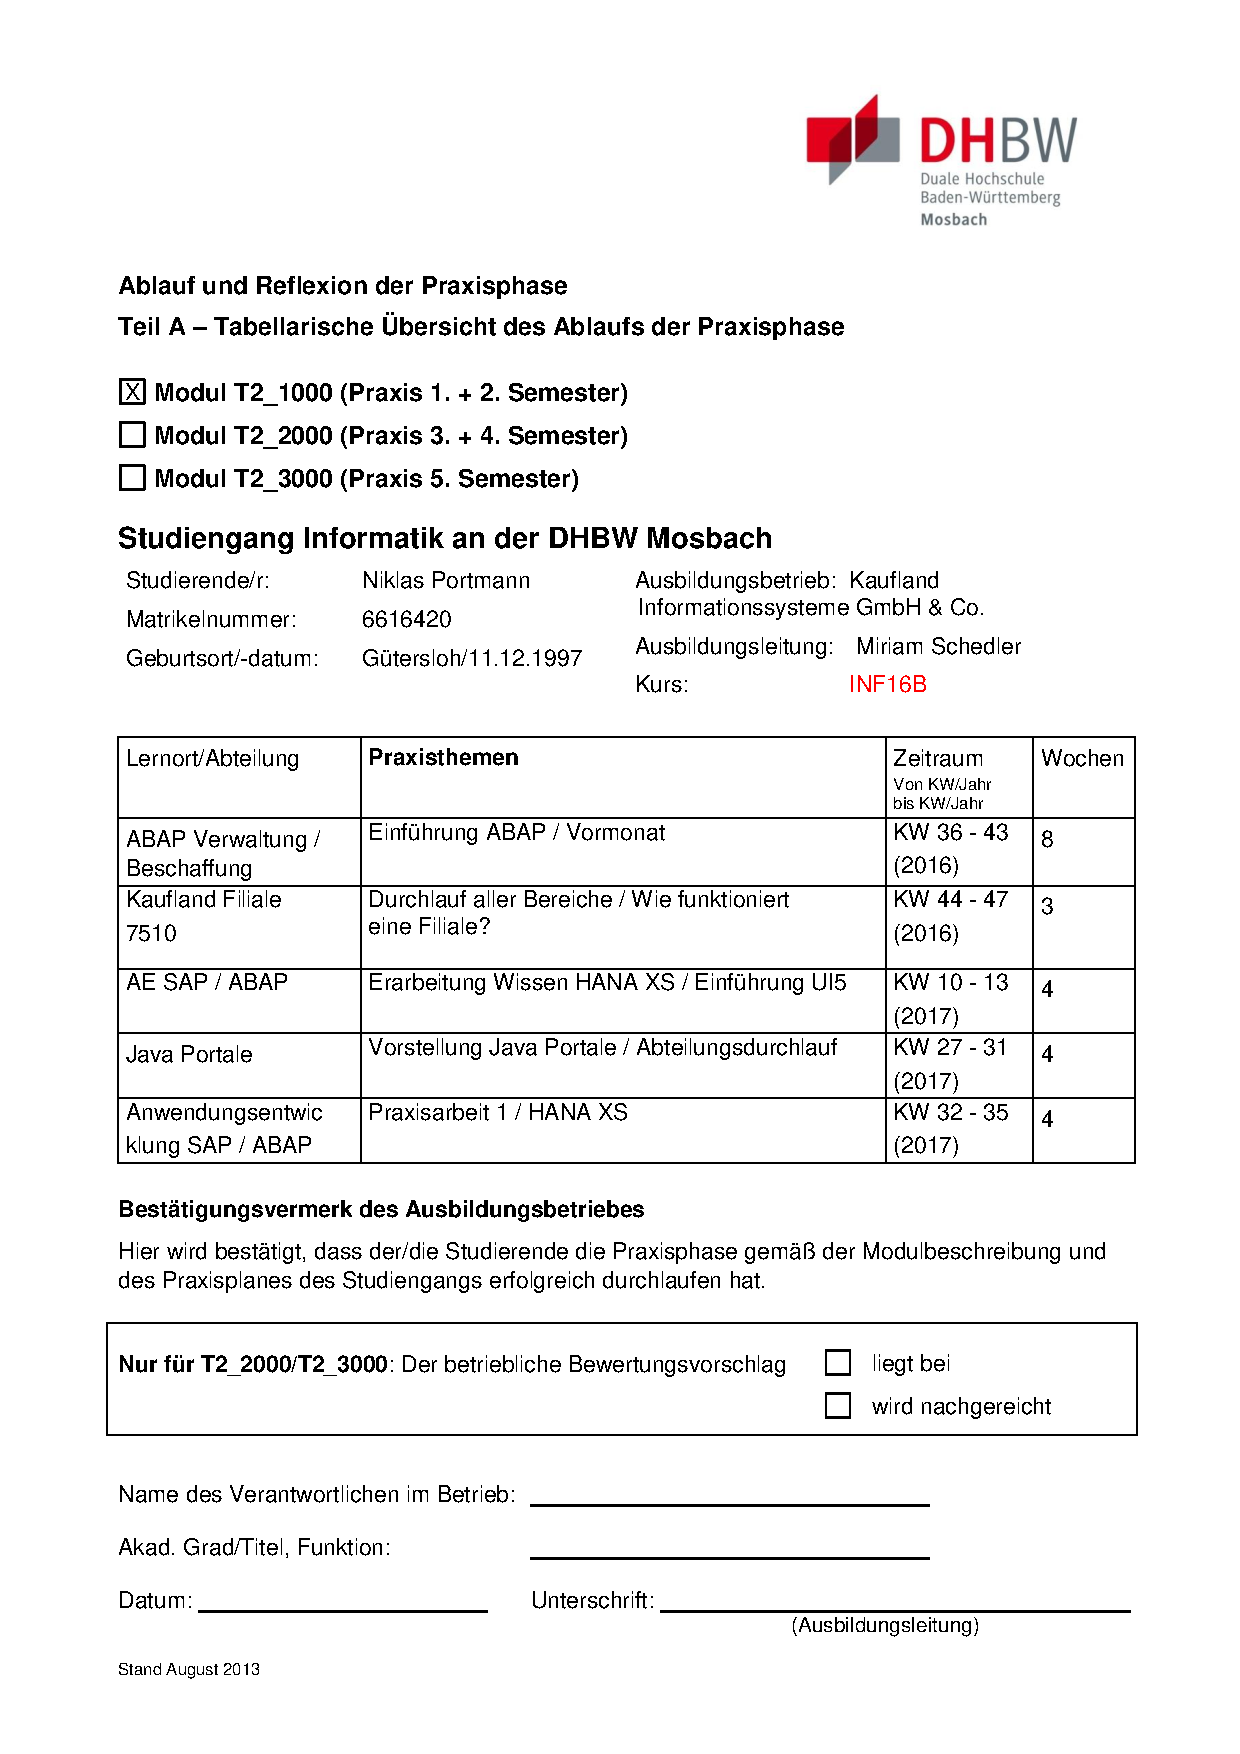
\includepdf[pages={1}]{include/Ablauf-Praxisphase1.pdf}

\tableofcontents

\chapter{Abkürzungsverzeichnis}

\begin{acronym}
    \acro{API}{Application Programming Interface}
    \acro{CIL}{Common Intermediate Language}
    \acro{DVCS}{Distributed Version Control System}
    \acro{KIS}{Kaufland Informationssysteme}
    \acro{MFP}{MyFitnessPal}    
    \acro{MVP}{Minimum Viable Product}
    \acro{ORM}{Object-Relational Mapping}
    \acro{PT}{Personentag}
    \acrodefplural{PT}[PT]{Personentage}
    \acro{SDK}{Software Development Kit}
    \acro{UI}{User Interface}
    \acro{UML}{Unified Modeling Language}
\end{acronym}

%\ac    K Desktop Environment (KDE)
%\acs   KDE
%\acl   K Desktop Environment

% add p to add plurals (s)


\mainmatter

% Einzelne Unterdateien in die Datei einlesen.
\chapter{Tabellen}

\section{Tabelle ohne Spalten}

\begin{tabular}{lcr}
    Spalte 1 & Spalte 2 & Spalte 3 \\
    1 & 2 & 3 \\
\end{tabular}

\section{Tabelle mit horizontalen Linien}

\begin{tabular}{l*{6}{c}r}
    \toprule
    Team              & P & W & D & L & F  & A & Pts \\
    \midrule
    Manchester United & 6 & 4 & 0 & 2 & 10 & 5 & 12  \\
    Celtic            & 6 & 3 & 0 & 3 &  8 & 9 &  9  \\
    Benfica           & 6 & 2 & 1 & 3 &  7 & 8 &  7  \\
    FC Copenhagen     & 6 & 2 & 1 & 3 &  5 & 8 &  7  \\
    \bottomrule
\end{tabular}

\section{Tabelle mit offener Seite}

\begin{center}
    \begin{tabular}{ | l | c | r }
      \hline
      1 & 2 & 3 \\ \hline
      4 & 5 & 6 \\ \hline
      7 & 8 & 9 \\
      \hline
    \end{tabular}
  \end{center}

\section{Tabelle von Niklas' PA}

\begin{table}[H]
    \centering
    \begin{tabular}{|p{0.25\linewidth}|p{0.7\linewidth}|}
      \hline
      Schlüsselwort & Beschreibung \\ \hline
      \code{SELECT} & Selektiert einen odere mehrere Datensätze aus einer Tabelle. \\
      \code{INSERT} & Fügt einen neuen Datensatz in eine Tabelle ein. \\
      \code{UPDATE} & Verändert Daten bereits bestehender Datensätze in einer Tabelle. \\
      \code{DELETE} & Löscht einen oder mehrere bestehenden Datensätze aus einer Tabelle. \\
      \code{(INNER) JOIN}   & Fügt Abfragen von zwei oder mehreren Tabellen zusammen.
            Auf das Schlüsselwort \code{JOIN} folgt nach dem Tabellennamen das Schlüsselwort
            \code{ON}. \\
      \code{ON} & Auf das Schlüsselwort folgt ein Vergleich. Zeilen die diesem Vergleich
            entsprechen, werden miteinander gejoint. Nur erfolgreich gejointe Zeilen werden
            selektiert, außer es wird ein \code{RIGHT/LEFT JOIN} benutzt. \\
      \code{RIGHT/LEFT JOIN} & Erfüllt die selbe Aufgabe wie der \code{INNER JOIN}.
            Je nach Schlüsselwort, werden auch Zeilen aus der Tabelle die rechts/links
            von dem Join selektiert, die nicht dem Vergleich hinter \code{ON} entsprechen. \\
      \hline
      \end{tabular}
      \caption{Auswahl diverser SQL Schlüsselwörter}
      \small{Die Tabelle zeigt in der linken Spalte die Schlüsselwörter und auf
      der rechten Seite die dazu gehörigen Beschreibungen.}
      \label{sql-keywords}
\end{table}

Referenzierung von der \Cref{sql-keywords} innerhalb eines Fließtexts.

Da die Erstellung von Tabellen kompliziert ist, kann man auf \href{https://www.tablesgenerator.com/}{www.tablesgenerator.com} sich eine Tabelle erstellen. Dieses \href{https://ei.hs-duesseldorf.de/personen/braun/lehre/Documents/LaTeX%20SS15/Latex%2010%20-%20Tabellen.pdf}{Skript} zeigt weitere Tabellenbefehle.
\chapter{Auflistungen}

\section{Auflistung}
\begin{itemize}
  \item erste Ebene
  \begin{itemize}
    \item[*)] zweite Ebene
    \begin{itemize}
      \item dritte Ebene
        \begin{itemize}
          \item vierte Ebene
        \end{itemize}
    \end{itemize}
  \end{itemize}
\end{itemize}


\section{Aufzählung}

\begin{enumerate}
  \item erste Ebene
  \begin{enumerate}
    \item zweite Ebene
    \begin{enumerate}
      \item dritte Ebene
      \begin{enumerate}
        \item vierte Ebene
      \end{enumerate}
    \end{enumerate}
  \end{enumerate}
\end{enumerate}

\noindent Es gibt auch weitere hilfreiche \href{https://www.namsu.de/Extra/befehle/Auflistungen.html}{Auflistungen}.
\chapter{Figures (Illustrationen)}

\begin{figure}[H]
    \centering
    
\includegraphics[width=0.25\textwidth]{images/kis}
    \caption{Kaufland Logo.}
    \small Das derzeitige Logo von Kaufland.
    \label{fig-kis-big}
\end{figure}

\vspace{15pt} % Vertikaler Abstand

\begin{figure}[H]
    %\centering
    \begin{subfigure}{.45\textwidth}
      \centering
      
\includegraphics[width=.325\linewidth]{images/kis}
      \caption{Kaufland Logo.}
      \label{fig-kis}
    \end{subfigure}%
    \hspace{1em} % Horizontaler Abstand
    \begin{subfigure}{.45\textwidth}
      \centering
      
\includegraphics[width=.9\linewidth]{images/sitios}
      \caption{SITIOS Logo.}
      \label{fig-sitios}
    \end{subfigure}

    \centering
    \caption{Mehrere Figures nebeneinander.}
    \small Illustrationen die zusammenhängen können nebeneinander mit jeweils einer kurzen Beschreibung dargestellt werden. Diese werden in diesem Text referenziert. \newline (a) ist Rot. (b) ist Grau. % \newline erzwingt Zeilenumbruch
    \label{fig-search}
\end{figure}
\chapter{Zitate und Quellenverweise}

Zitate können mit verschiedenen Befehlen erzeugt werden. Beispiel: \parencite{diadoc} \compcite{hanaxsdifference}

\noindent Siehe auch \href{https://anjalorenz.wordpress.com/2012/02/14/biblatex-kurz-im-ueberblick/}{Biblatex Zitierungsbefehle}.

In den anderen Kapiteln wurden auch schon Tabellen und Figuren referenziert in den Texten. Dafür muss in der Figur/der Tabelle ein label erzeugt werden mit \code{\textbackslash{}label\{label\}}, und dieses kann dann mit \code{\textbackslash{}Cref\{label\}}.

\nocite{*}

\backmatter

\sloppy

\cleardoublepage
\phantomsection
\addcontentsline{toc}{chapter}{Literatur}
\printbibliography

\end{document}
